\documentclass[titlepage,11pt]{article}
\usepackage{comment}
\usepackage{enumitem}
\usepackage{listings}
\usepackage{amsmath}
\usepackage{graphicx}
\usepackage[font=small,labelfont=bf]{caption}
\usepackage[bahasa]{babel}
\usepackage{float}
\usepackage{verbatim}
\usepackage{graphicx,tabularx,multirow}
\usepackage{xcolor}
\usepackage[onehalfspacing]{setspace}
\usepackage[
	allcolors=visigrey,
	colorlinks=true,
]{hyperref}
\usepackage[a4paper,left=2cm,right=2cm]{geometry}
% Pengaturan kutipan artikel
\usepackage[style=ieee, backend=biber]{biblatex}
%Code listing style pak akok
\definecolor{codegreen}{rgb}{0,0.6,0}
\definecolor{codegray}{rgb}{0.5,0.5,0.5}
\definecolor{codepurple}{rgb}{0.58,0,0.82}
\definecolor{backcolour}{rgb}{0.95,0.95,0.92}

\lstdefinestyle{mystyle}{
	backgroundcolor=\color{backcolour}, commentstyle=\color{codegreen},
	keywordstyle=\color{magenta},
	numberstyle=\small\color{codegray},
	stringstyle=\color{codepurple},
	basicstyle=\ttfamily\footnotesize,
	breakatwhitespace=false,         
	breaklines=true,                 
	captionpos=t,                    
	keepspaces=true,                 
	numbers=left,                    
	numbersep=5pt,                  
	showspaces=false,                
	showstringspaces=false,
	showtabs=false,           
	frame = single,
	tabsize=2
}
\lstset{style=mystyle}

\definecolor{visigrey}{rgb}{.1,.15,.15}
\geometry{top=1cm,bottom=.5cm}
\savegeometry{titlepage}
\geometry{top=2cm,bottom=2cm}
\savegeometry{main}

\def\bspace{\(\qquad\qquad\qquad\)}
\usepackage[T1]{fontenc}
\usepackage[utf8]{inputenc}
\usepackage{tgheros}
\renewcommand*\familydefault{\sfdefault}

\setcounter{tocdepth}{6}

\def\autor{Laboratorium }
\def\lab{Multimedia dan Internet of Things}
\def\departemen{Departemen Teknik Komputer}
\def\institut{Institut Teknologi Sepuluh Nopember}
\def\praktikum{Praktikum \\ Jaringan Komputer}
\def\nama{Cedric Anthony Edysa - 5024221015 \\ Larasati Lituhayu - 5024221025 \\ Azaria Putri Fawnia - 5024221038\\Vania Bunga Febrina - 5024221069}
% Ubah Judul sesuai dengan modul
\def\judul{Routing Static dan Routing Dinamis (Mikrotik)}
\def\tanggal{2024}
\begin{document}
% Ubah Bahasa sesuai dengan keinginan
\selectlanguage{bahasa}

\def\headingtype{\bf \small}
\loadgeometry{titlepage}
\begin{titlepage}
	\centering
	\begin{tabularx}{\textwidth}{Xr}
		\multirow[c]{6}{*}{
\includegraphics[width=3cm]{Cover/img/logodepart.png}} & {\emph{\headingtype \autor}}    \\ [-2pt]
		                                                                          & {\headingtype \lab}             \\[-2pt]
		                                                                          & {\headingtype \departemen}      \\[-2pt]
		                                                                          & {\headingtype \emph{\institut}} \\[-2pt]
		\vspace{1.6cm}
	\end{tabularx}\par
	\vspace{5.0cm}
	{\Huge \bf  \praktikum \par}
	\vspace{2.0cm}
	{\LARGE \bf \judul \par}
	\vspace{2.0cm}
	{\Large \nama \par}
	\vfill
	{\Large \tanggal \par}
	\vfill
	{\centering
		
\includegraphics[width=\textwidth]{Cover/img/footer.png}
	}
\end{titlepage}
\loadgeometry{main}
% Pilih Modul yang akan di build
\section{Pendahuluan}
Pada Wireless Jaringan Komputer, terdapat setidaknya 3 jenis, yaitu Point-to-Point Protocol (PPP),
Point-to-multipoint dan Wireless Bridging. 
\\ \\ \indent Point-to-Point Protocol (PPP) adalah data link protokol yang umum digunakan dalam membangun 
hubungan langsung antara dua node jaringan. Hal ini dapat menyediakan koneksi otentikasi, transmisi enkripsi (menggunakan ECP, RFC 1968), dan kompresi. 
Jenis ini biasanya digunakan untuk menghubungkan jaringan antar 2 gedung atau antar 2 BTS (Base Transceiver Station).
\\ \\ \indent Point-to-multipoint adalah pendekatan yang paling populer untuk komunikasi nirkabel yang memiliki banyak node, tujuan akhir atau pengguna akhir. 
Jenis ini biasanya digunakan untuk membuat wifi atau hotspot yang berasal dari 1 sumber disebar ke banyak client dalam suatu jaringan.
\\ \\ \indent Wireless Bridging digunakan untuk menghubungkan dua segmen LAN melalui tautan nirkabel. Kedua
segmen akan berada di subnet yang sama dan terlihat seperti dua switch Ethernet yang dihubungkan
oleh kabel ke semua komputer di subnet.
\\ \\ \indent Untuk mengembangkan jaringan komputer berbasis wireless yang berkualitas dan mempunyai ketersediaan tinggi, penggunaan 3 jenis ini perlu disesuaikan dengan kebutuhan dan kondisi nya, sehingga
kali ini akan dibahas satu persatu dari 3 jenis koneksi wireless tersebut.
%===========================================================%

\section{Tujuan Praktikum}
Mengetahui dan memahami 3 jenis koneksi pada Jaringan Wireless.
Diharapkan praktikan Dapat mengkonfigurasi koneksi Wireless Bridge, Point to Point dan Point to Multipoint dengan tepat
%===========================================================%

\section{Alat dan Bahan}
\begin{itemize}[label=$\bullet$, itemsep=-1pt, leftmargin=*]
	\item 2 atau lebih perangkat router mikrotik yang sudah support wireless.
	\item Aplikasi Winbox.
\end{itemize}
%===========================================================%

\section{Langkah-langkah Percobaan}
\textbf{gambar pada langkah-langkah di bagian ini akan diisi gambar contoh dari template dulu,
		karena nanti akan kami ganti dengan screenshot langkah-langkah kami saat praktikum}
\subsection{Wireless Point to Point}
Untuk koneksi Point to Point seperti contohnya topologi seperti dibawah ini, biasanya digunakan untuk
menghubungkan 2 router atau 2 node jaringan, Hal ini dilakukan biasanya untuk koneksi koneksi
jarak jauh yang mengharapkan kecepatan tinggi misal untuk menghubungkan jaringan antar gedung,
menghubungkan BTS (Base Transceiver Station) to BTS (Base Transceiver Station). Koneksi point
to point ini akan lebih aman karena maksimal node yang terhubung hanya 2. Untuk konfigurasinya
seperti berikut ini.\\ \\

%Langkah untuk konfigurasi Router 1
\begin{center} 
	\textbf{Konfigurasi Router 1}
\end{center}

\begin{enumerate}
	% poin 1
	\item Buka aplikasi WinBox pada PC 1 dan lakukan koneksi ke Router 1.
	\\Neighbors > Refresh > Double click Router yang terdeteksi > Connect
	\begin{figure}[H]
		\centering
		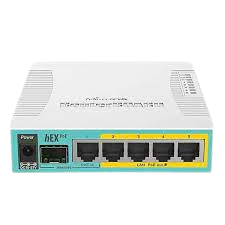
\includegraphics[width=0.5\linewidth]{P1/img/contoh.png}
		\caption{Step 1}
		\label{fig:gambar1}
	\end{figure}

	% poin 2
	\item Berikan IP address pada interface wlan 1 yang dapat dibuat pada tab IP > Addresses.
	\begin{figure}[H]
		\centering
		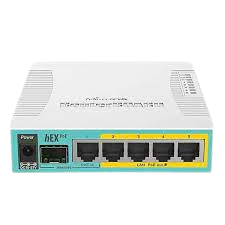
\includegraphics[width=0.5\linewidth]{P1/img/contoh.png}
		\caption{Step 2.1}
		\label{fig:gambar2}
	\end{figure}

	% poin 3
	\item Berikan IP address sesuai dengan cara pengaturan IP address yang benar. Berikan IP address
	yang berbeda dengan contoh di modul.
	\begin{figure}[H]
		\centering
		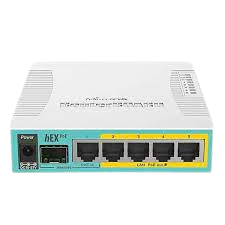
\includegraphics[width=0.5\linewidth]{P1/img/contoh.png}
		\caption{Step 2.2}
		\label{fig:gambar3}
	\end{figure}

	% poin 4
	\item Atur Router 1 untuk mengaktifkan WLAN pada tab Wireless, pilih wlan1, lalu klik tombol centang.
	Kemudian atur WLAN pada mode bridge dan isi SSID yang diinginkan. Berikan SSID sekreatif
	mungkin, yang berbeda dengan contoh di modul.
	
	\begin{figure}[H]
		\centering
		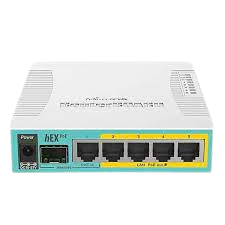
\includegraphics[width=0.5\linewidth]{P1/img/contoh.png}
		\caption{Step 3}
		\label{fig:gambar4}
	\end{figure}

\end{enumerate}

%Langkah untuk konfigurasi Router 2
\begin{center} 
	\textbf{Konfigurasi Router 2}
\end{center}

\begin{enumerate}
	% poin 1
	\item Buka WinBox dan lakukan koneksi ke Router
	\begin{figure}[H]
		\centering
		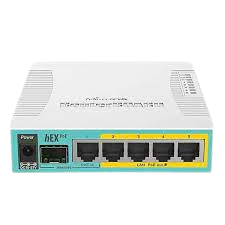
\includegraphics[width=0.5\linewidth]{P1/img/contoh.png}
		\caption{Step 1}
		\label{fig:gambar5}
	\end{figure}

	% poin 2
	\item Berikan IP address pada interface wlan 1 yang dapat dibuat pada tab IP > Addresses. Berikan
	IP address sesuai dengan cara pengaturan IP address yang benar. Berikan IP address yang
	berbeda dengan contoh di modul.
	\begin{figure}[H]
		\centering
		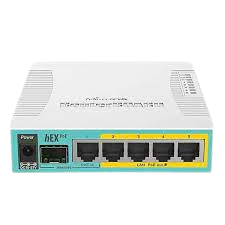
\includegraphics[width=0.5\linewidth]{P1/img/contoh.png}
		\caption{Step 2}
		\label{fig:gambar6}
	\end{figure}

	% poin 3
	\item Atur Router 2 untuk mengaktifkan WLAN pada tab Wireless, pilih wlan1, lalu klik tombol centang.
	Kemudian atur WLAN pada mode station. Kemudian cari sinyal yang sudah dipancarkan oleh
	Router 1, sesuai dengan nama SSID yang sudah dibuat
	\begin{figure}[H]
		\centering
		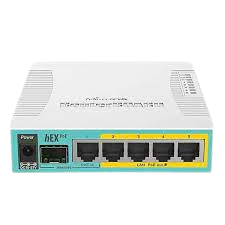
\includegraphics[width=0.5\linewidth]{P1/img/contoh.png}
		\caption{Step 3}
		\label{fig:gambar7}
	\end{figure}

\end{enumerate}

%Langkah untuk Mengecek keberhasilan konfigurasi
\begin{center} 
	\textbf{Mengecek keberhasilan konfigurasi}
\end{center}

\begin{enumerate}
	% poin 1
	\item Lakukan test ping dari Router 1 ke Router 2
	\begin{figure}[H]
		\centering
		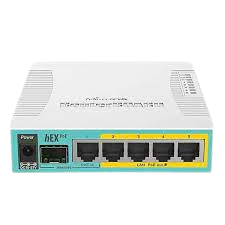
\includegraphics[width=0.5\linewidth]{P1/img/contoh.png}
		\caption{Step 1}
		\label{fig:gambar8}
	\end{figure}

	% poin 2
	\item Lakukan test ping dari Router 2 ke Router 1
	\begin{figure}[H]
		\centering
		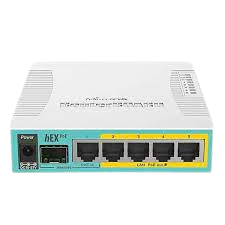
\includegraphics[width=0.5\linewidth]{P1/img/contoh.png}
		\caption{Step 2}
		\label{fig:gambar9}
	\end{figure}

\end{enumerate}

\subsection{Wireless Point to Multipoint}
Koneksi ini yang paling banyak digunakan, karena kelebihannya yaitu dapat mengkoneksikan multipoint atau banyak node dari satu point atau node sumber, penerapan pada koneksi ini biasanya berupa
hotspot. Untuk konfigurasinya seperti berikut. Untuk gambar topologi sama dengan PointToPoint,
hanya saja berbeda di konfigurasi dan mode pada routernya.

%Langkah untuk konfigurasi Router 1
\begin{center} 
	\textbf{Konfigurasi Router 1}
\end{center}

\begin{enumerate}
	% poin 1
	\item Berikan IP address sesuai dengan cara pengaturan IP address yang benar. Berikan IP address
	yang berbeda dengan contoh di modul.	
	\begin{figure}[H]
		\centering
		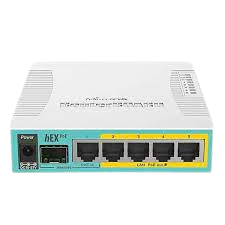
\includegraphics[width=0.5\linewidth]{P1/img/contoh.png}
		\caption{Step 1}
		\label{fig:gambar10}
	\end{figure}

	% poin 2
	\item Atur Router 1 untuk mengaktifkan WLAN pada tab Wireless, pilih wlan1, lalu klik tombol centang. Kemudian atur WLAN pada mode ap bridge dan isi SSID yang diinginkan. Berikan SSID
	sekreatif mungkin, yang berbeda dengan contoh di modul.
	\begin{figure}[H]
		\centering
		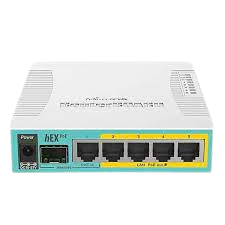
\includegraphics[width=0.5\linewidth]{P1/img/contoh.png}
		\caption{Step 2}
		\label{fig:gambar11}
	\end{figure}

\end{enumerate}

%Langkah untuk konfigurasi Router 2
\begin{center} 
	\textbf{Konfigurasi Router 2}
\end{center}

\begin{enumerate}
	% poin 1
	\item Berikan IP address pada interface wlan 1 yang dapat dibuat pada tab IP > Addresses. Berikan
	IP address sesuai dengan cara pengaturan IP address yang benar. Berikan IP address yang
	berbeda dengan contoh di modul.
	\begin{figure}[H]
		\centering
		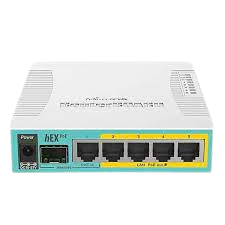
\includegraphics[width=0.5\linewidth]{P1/img/contoh.png}
		\caption{Step 1}
		\label{fig:gambar12}
	\end{figure}

	% poin 2
	\item . Atur Router 2 untuk mengaktifkan WLAN pada tab Wireless, pilih wlan1, lalu klik tombol centang. 
	Kemudian atur WLAN pada mode station bridge. Kemudian cari sinyal yang sudah dipancarkan
	oleh Router 1, sesuai dengan nama SSID yang sudah dibuat
	
	\begin{figure}[H]
		\centering
		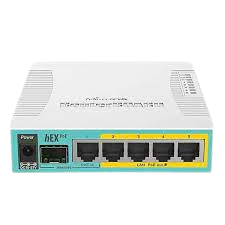
\includegraphics[width=0.5\linewidth]{P1/img/contoh.png}
		\caption{Step 2}
		\label{fig:gambar13}
	\end{figure}

\end{enumerate}

%Langkah untuk Mengecek keberhasilan konfigurasi
\begin{center} 
	\textbf{Mengecek keberhasilan konfigurasi}
\end{center}

\begin{enumerate}
	% poin 1
	\item Lakukan test ping dari Router 1 ke Router 2
	\begin{figure}[H]
		\centering
		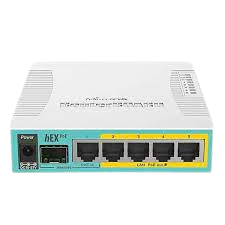
\includegraphics[width=0.5\linewidth]{P1/img/contoh.png}
		\caption{Step 1}
		\label{fig:gambar14}
	\end{figure}

	% poin 2
	\item Lakukan test ping dari Router 2 ke Router 1
	\begin{figure}[H]
		\centering
		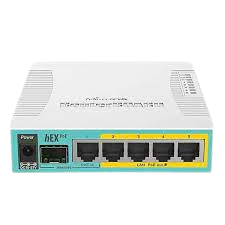
\includegraphics[width=0.5\linewidth]{P1/img/contoh.png}
		\caption{Step 2}
		\label{fig:gambar15}
	\end{figure}

\end{enumerate}

\subsection{Wireless Bridge}
Untuk wireless bridge ini sangatlah sederhana, koneksi ini sangat jarang ditemui pada implementasi realnya, konfigurasi ini menjadikan seolah-olah koneksi yang terhubung menggunakan switch,
keunggulan yang saya rasakan yaitu ringannya kinerja router yang menggunakan koneksi ini. Untuk konfigurasinya seperti berikut. Untuk gambar topologi sama dengan Point To Point, hanya saja
berbeda di konfigurasi dan mode pada routernya.

%Langkah untuk konfigurasi Router 1
\begin{center} 
	\textbf{Konfigurasi Router 1}
\end{center}

\begin{enumerate}
	% poin 1
	\item Buka WinBox dan lakukan koneksi ke Router.
	\begin{figure}[H]
		\centering
		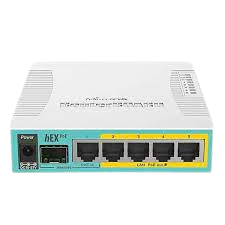
\includegraphics[width=0.5\linewidth]{P1/img/contoh.png}
		\caption{Step 1}
		\label{fig:gambar16}
	\end{figure}

	% poin 2
	\item Berikan IP address pada interface wlan1 dan ethernet 2 yang dapat dibuat pada tab IP > Addresses. Berikan IP address sesuai dengan cara pengaturan IP address yang benar. Berikan IP
	address yang berbeda dengan contoh di modul.
	\begin{figure}[H]
		\centering
		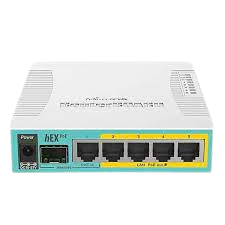
\includegraphics[width=0.5\linewidth]{P1/img/contoh.png}
		\caption{Step 2}
		\label{fig:gambar17}
	\end{figure}

	% poin 3
	\item Atur Router 1 untuk mengaktifkan WLAN pada tab Wireless, pilih wlan1, lalu klik tombol centang.
	Kemudian atur WLAN pada mode bridge dan isi SSID yang diinginkan. Berikan SSID sekreatif
	mungkin, yang berbeda dengan contoh di modul.
	
	\begin{figure}[H]
		\centering
		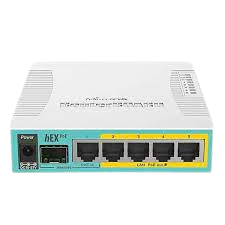
\includegraphics[width=0.5\linewidth]{P1/img/contoh.png}
		\caption{Step 1}
		\label{fig:gambar18}
	\end{figure}

	% poin 4
	\item Tambahkan bridge pada Router 1 untuk menghubungkan interface wlan1 dan ether 2. Buat
	bridge pada tab Bridge dan beri nama yang diinginkan.	
	\begin{figure}[H]
		\centering
		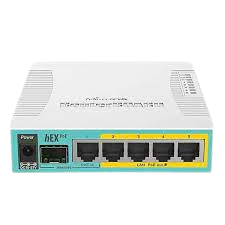
\includegraphics[width=0.5\linewidth]{P1/img/contoh.png}
		\caption{Step 2}
		\label{fig:gambar19}
	\end{figure}

	% poin 5
	\item Selanjutnya tambahkan port interface yang akan dihubungkan pada tab Ports, dan tambahkan
	interface wlan1 dan ehter2 pada bridge sesuai yang telah dibuat sebelumnya.
	\begin{figure}[H]
		\centering
		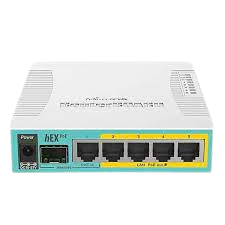
\includegraphics[width=0.5\linewidth]{P1/img/contoh.png}
		\caption{Step 1}
		\label{fig:gambar20}
	\end{figure}

	% poin 6
	\item Atur IP pada PC 1 dengan mengubah pengaturan pada setting ethernet. Ubah IP perangkat
	yang otomatis menjadi manual, pastikan IP PC 1 masih satu jaringan dengan IP lokal yang
	diinginkan, isi Gateway dengan IP Router yang tersambung dengan PC. Berikan IP address
	yang berbeda dengan contoh yang ada di modul.
	\begin{figure}[H]
		\centering
		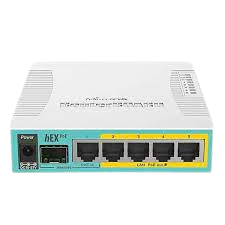
\includegraphics[width=0.5\linewidth]{P1/img/contoh.png}
		\caption{Step 2}
		\label{fig:gambar21}
	\end{figure}

\end{enumerate}


%Langkah untuk konfigurasi Router 2
\begin{center} 
	\textbf{Konfigurasi Router 2}
\end{center}

\begin{enumerate}
	% poin 1
	\item Buka WinBox dan lakukan koneksi ke Router
	\begin{figure}[H]
		\centering
		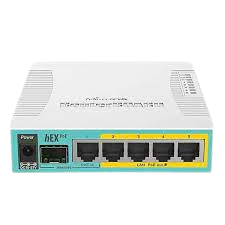
\includegraphics[width=0.5\linewidth]{P1/img/contoh.png}
		\caption{Step 1}
		\label{fig:gambar22}
	\end{figure}

	% poin 2
	\item Berikan IP address pada interface wlan1 dan ethernet 2 yang dapat dibuat pada tab IP > Addresses. Berikan IP address sesuai dengan cara pengaturan IP address yang benar. Berikan IP
	address yang berbeda dengan contoh di modul.
	\begin{figure}[H]
		\centering
		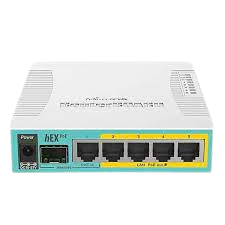
\includegraphics[width=0.5\linewidth]{P1/img/contoh.png}
		\caption{Step 2}
		\label{fig:gambar23}
	\end{figure}

	% poin 3
	\item Atur Router 2 untuk mengaktifkan WLAN pada tab Wireless, pilih wlan1, lalu klik tombol centang. Kemudian atur WLAN pada mode station pseudobridge. Kemudian cari sinyal yang sudah
	dipancarkan oleh Router 1, sesuai dengan nama SSID yang sudah dibuat.
	\begin{figure}[H]
		\centering
		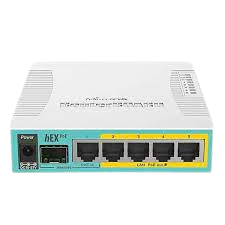
\includegraphics[width=0.5\linewidth]{P1/img/contoh.png}
		\caption{Step 1}
		\label{fig:gambar24}
	\end{figure}

	% poin 4
	\item Tambahkan bridge pada Router 2 untuk menghubungkan interface wlan1 dan ether 2. Buat
	bridge pada tab Bridge dan beri nama yang diinginkan.
	\begin{figure}[H]
		\centering
		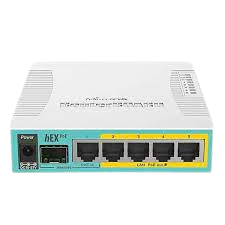
\includegraphics[width=0.5\linewidth]{P1/img/contoh.png}
		\caption{Step 2}
		\label{fig:gambar25}
	\end{figure}

	% poin 5
	\item Selanjutnya tambahkan port interface yang akan dihubungkan pada tab Ports, dan tambahkan
	interface wlan1 dan ehter2 pada bridge sesuai yang telah dibuat sebelumnya.
	\begin{figure}[H]
		\centering
		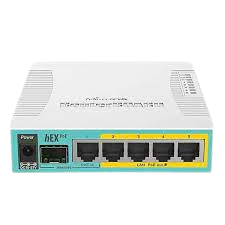
\includegraphics[width=0.5\linewidth]{P1/img/contoh.png}
		\caption{Step 1}
		\label{fig:gambar26}
	\end{figure}

	% poin 6
	\item Atur IP pada PC 2 dengan mengubah pengaturan pada setting ethernet. Ubah IP perangkat
	yang otomatis menjadi manual, pastikan IP PC 2 masih satu jaringan dengan IP lokal yang
	diinginkan, isi Gateway dengan IP Router yang tersambung dengan PC. Berikan IP address
	yang berbeda dengan contoh yang ada di modul.
	\begin{figure}[H]
		\centering
		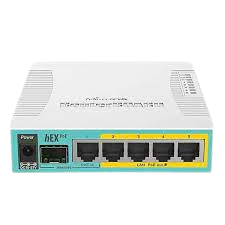
\includegraphics[width=0.5\linewidth]{P1/img/contoh.png}
		\caption{Step 2}
		\label{fig:gambar27}
	\end{figure}

\end{enumerate}

%Langkah untuk Mengecek keberhasilan konfigurasi
\begin{center} 
	\textbf{Mengecek keberhasilan konfigurasi}
\end{center}

\begin{enumerate}
	% poin 1
	\item Lakukan test ping dari PC 1 ke PC 2
	\begin{figure}[H]
		\centering
		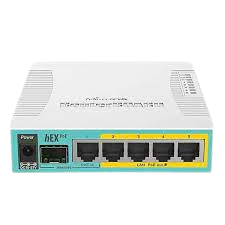
\includegraphics[width=0.5\linewidth]{P1/img/contoh.png}
		\caption{Step 1}
		\label{fig:gambar28}
	\end{figure}

	% poin 2
	\item Lakukan test ping dari PC 2 ke PC 1
	\begin{figure}[H]
		\centering
		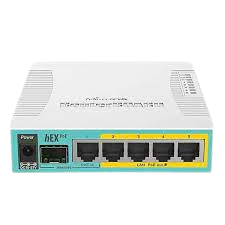
\includegraphics[width=0.5\linewidth]{P1/img/contoh.png}
		\caption{Step 2}
		\label{fig:gambar29}
	\end{figure}

	% poin 3
	\item Jika ping antar PC tidak berhasil, coba ulang setelah mematikan Firewall Public PC anda.
	\begin{figure}[H]
		\centering
		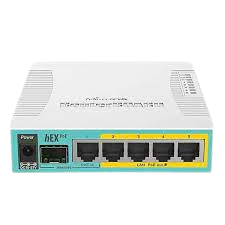
\includegraphics[width=0.5\linewidth]{P1/img/contoh.png}
		\caption{Step 1}
		\label{fig:gambar30}
	\end{figure}


\end{enumerate}


\section{Hasil Percobaan}
Hasil dari percobaan yang sudah kamu buat
%===========================================================%

\section{Kesimpulan}
simpulkan
%===========================================================%

\section{Lampiran}

\subsection{Tugas Pendahuluan}
\begin{enumerate}
	\item Buatlah topologi jaringan percobaan 1, 2, dan 3!
	\begin{itemize}
		\item Topologi jaringan percobaan 1
		\begin{figure}[H]
		\centering
		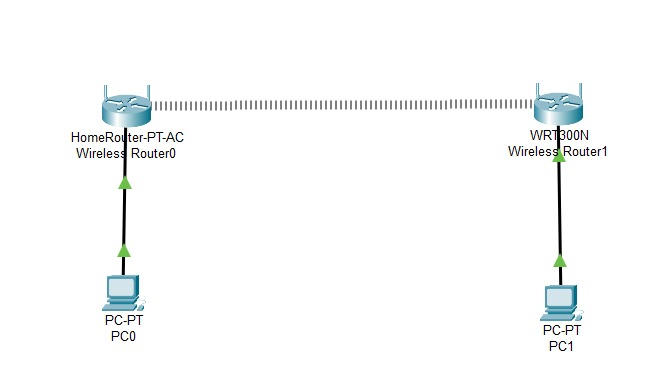
\includegraphics[width=0.7\linewidth]{P1/img/topologi1.jpg}
		\caption{Topologi Jaringan Percobaan 1}
		\label{fig:gambar31}
	\end{figure}


	\end{itemize}
	\begin{itemize}
		\item Topologi jaringan percobaan 2
		\begin{figure}[H]
			\centering
			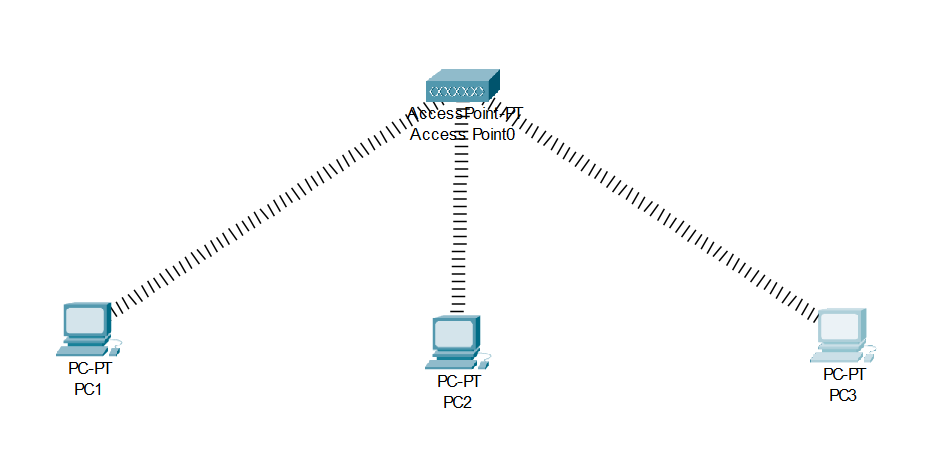
\includegraphics[width=0.7\linewidth]{P1/img/topologi2.png}
			\caption{Topologi Jaringan Percobaan 2}
			\label{fig:gambar32}
		\end{figure}
	\end{itemize}
	\begin{itemize}
		\item Topologi jaringan percobaan 3
		\begin{figure}[H]
			\centering
			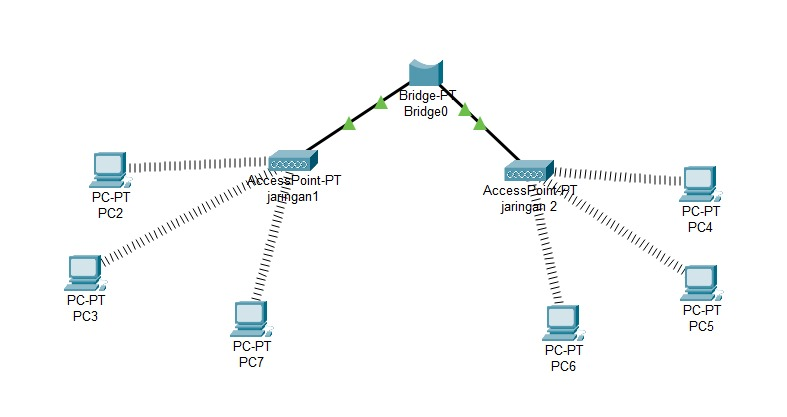
\includegraphics[width=0.7\linewidth]{P1/img/topologi3.jpg}
			\caption{Topologi Jaringan Percobaan 3}
			\label{fig:gambar33}
		\end{figure}
	\end{itemize}

	\item Perbedaan Point-to-Point, Point-to-Multipoint, dan Wireless Bridging
	\begin{itemize}
		\item Point-to-Point
		\begin{itemize}
			\item Point to point adalah metode pendistribusian akses internet yang hanya melibatkan 2 site saja.
			\item Hanya terdapat 1 radio station yang terkoneksi ke access point.
			\item Topologi PTP umumnya dipakai oleh ISP untuk mendistribusikan akses internet dari POP. 
			\item Kelebihan PTP adalah jaringan lebih stabil karena access point hanya akan memancarkan signalnya ke satu station saja, sehingga throughput yang dihasilkan akan maksimal. 
			\item Antena yang dipakai biasanya antena yang memiliki sudut pancaran 45-180 derajat (antena sectoral) atau 360 derajat (antena omni).
		\end{itemize}

		\item Point-to-Multipoint
		\begin{itemize}
			\item Menghubungkan satu access point ke beberapa station sekaligus
			\item PTMP biasanya dipakai untuk menekan biaya, karena hanya dengan satu radio access point saja sudah bisa mengkoneksikan beberapa radio station sekaligus. 
			\item Antena yang dipakai biasanya antena yang memiliki sudut pancaran 45-180 derajat (antena sectoral).
		\end{itemize}

		\item Wireless Bridging
		\begin{itemize}
			\item teknologi yang menghubungkan dua jaringan wireless yang berbeda, sehingga memungkinkan perangkat yang terhubung ke salah satu jaringan untuk dapat mengakses jaringan lainnya tanpa menggunakan kabel
			\item Wireless bridging dapat menghubungkan lebih dari 200 perangkat nirkabel secara bersamaan. 
			\item Fungsi Bridge juga mampu memindahkan data melalui intermediate network dengan tipe protokol sama sekali berbeda. 
			\item Bridge nirkabel memiliki fungsi yang lebih rumit dan berat ketimbang dua jenis Bridge yang sebelumnya.
		\end{itemize}
		
	\end{itemize}

	\item Follow IG Lab MIOT
	\begin{figure}[H]
		\centering
		\begin{subfigure}{0.3\linewidth}
			\centering
			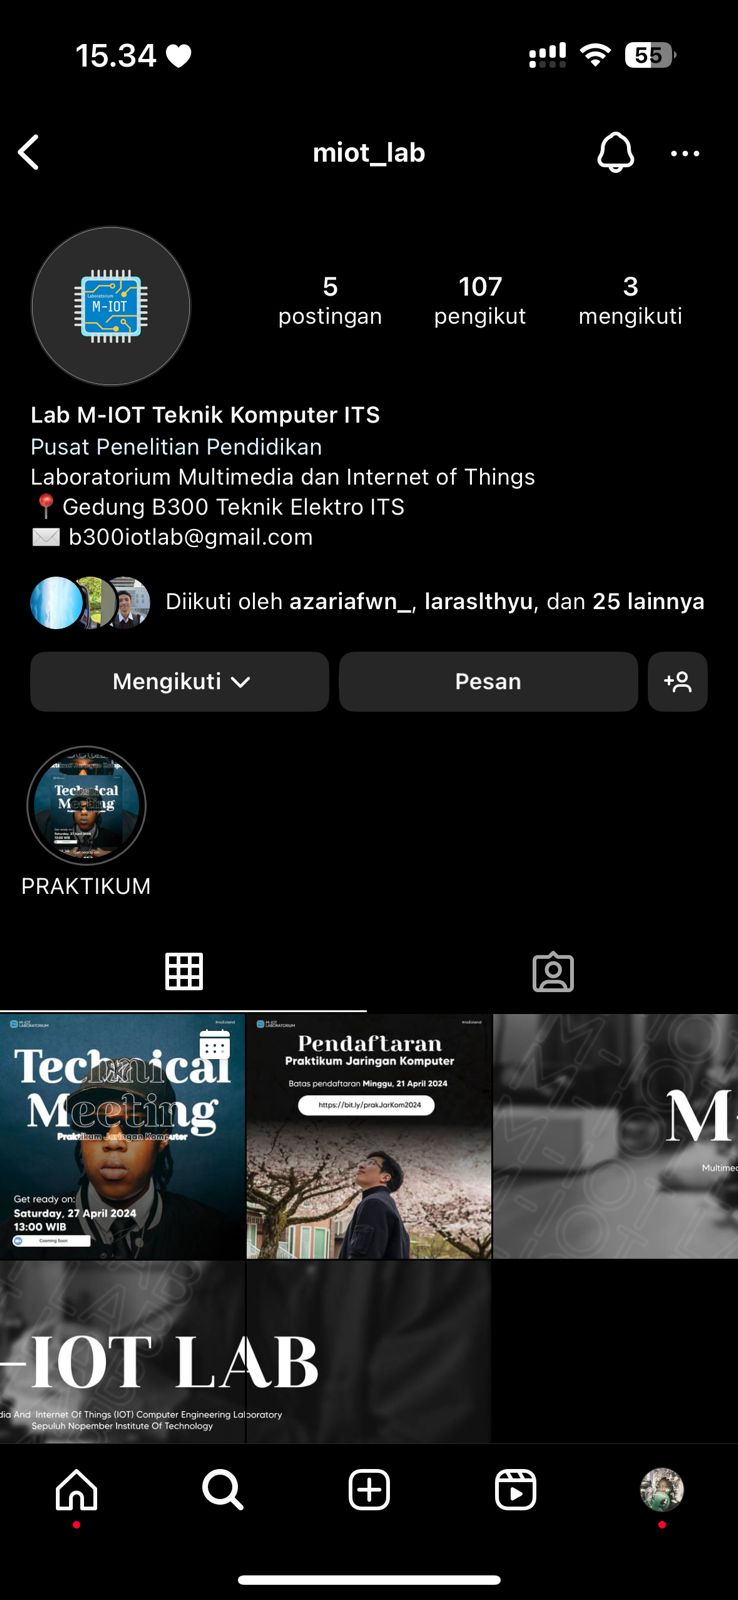
\includegraphics[width=\linewidth]{P1/img/vanfollow.jpg}
			\caption{Bukti Vania follow}
			\label{fig:gambar34}
		\end{subfigure}
		\begin{subfigure}{0.3\linewidth}
			\centering
			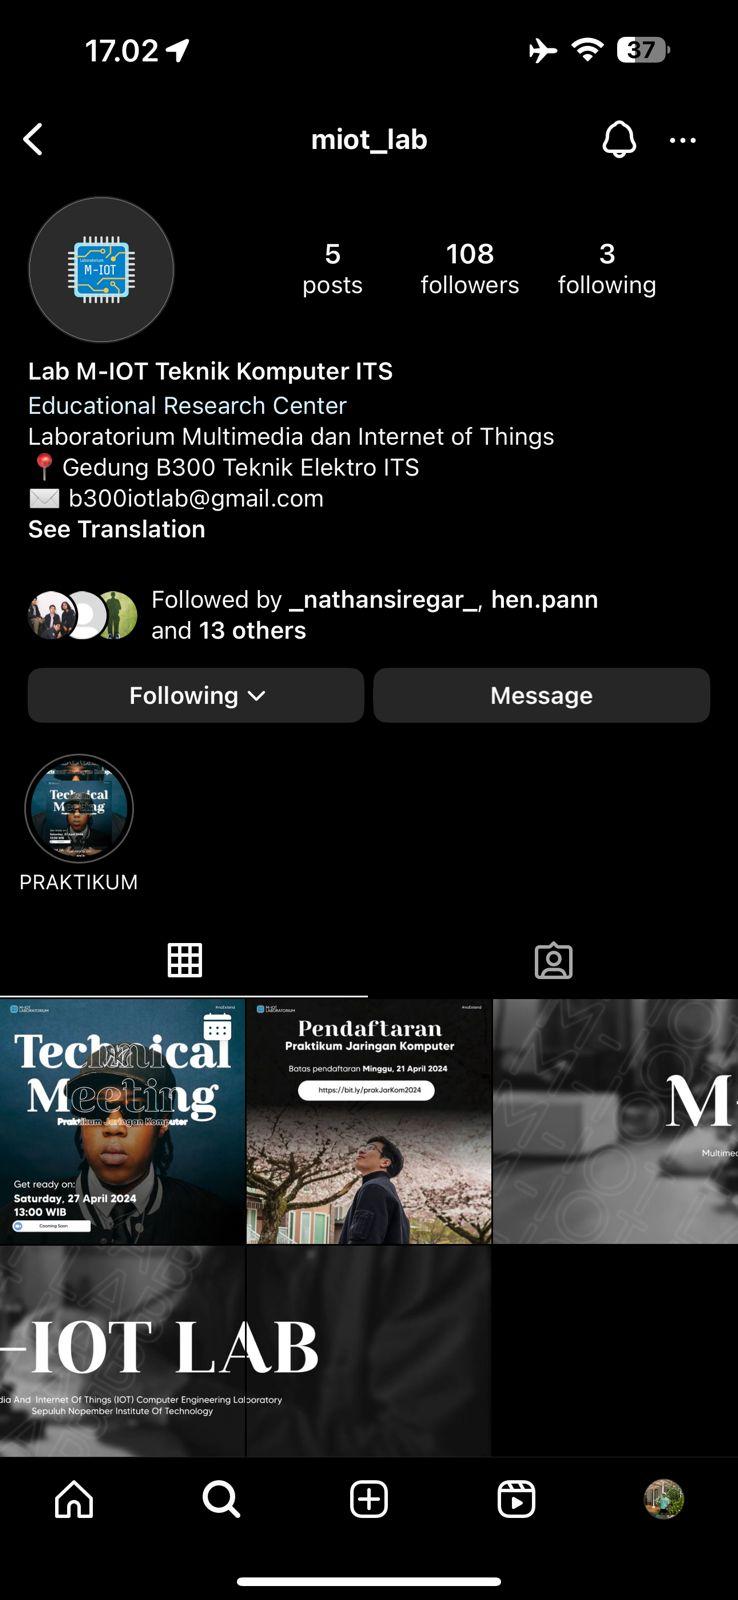
\includegraphics[width=\linewidth]{P1/img/cedfollow.jpg}
			\caption{Bukti Cedric follow}
			\label{fig:gambar35}
		\end{subfigure}
		\begin{subfigure}{0.3\linewidth}
			\centering
			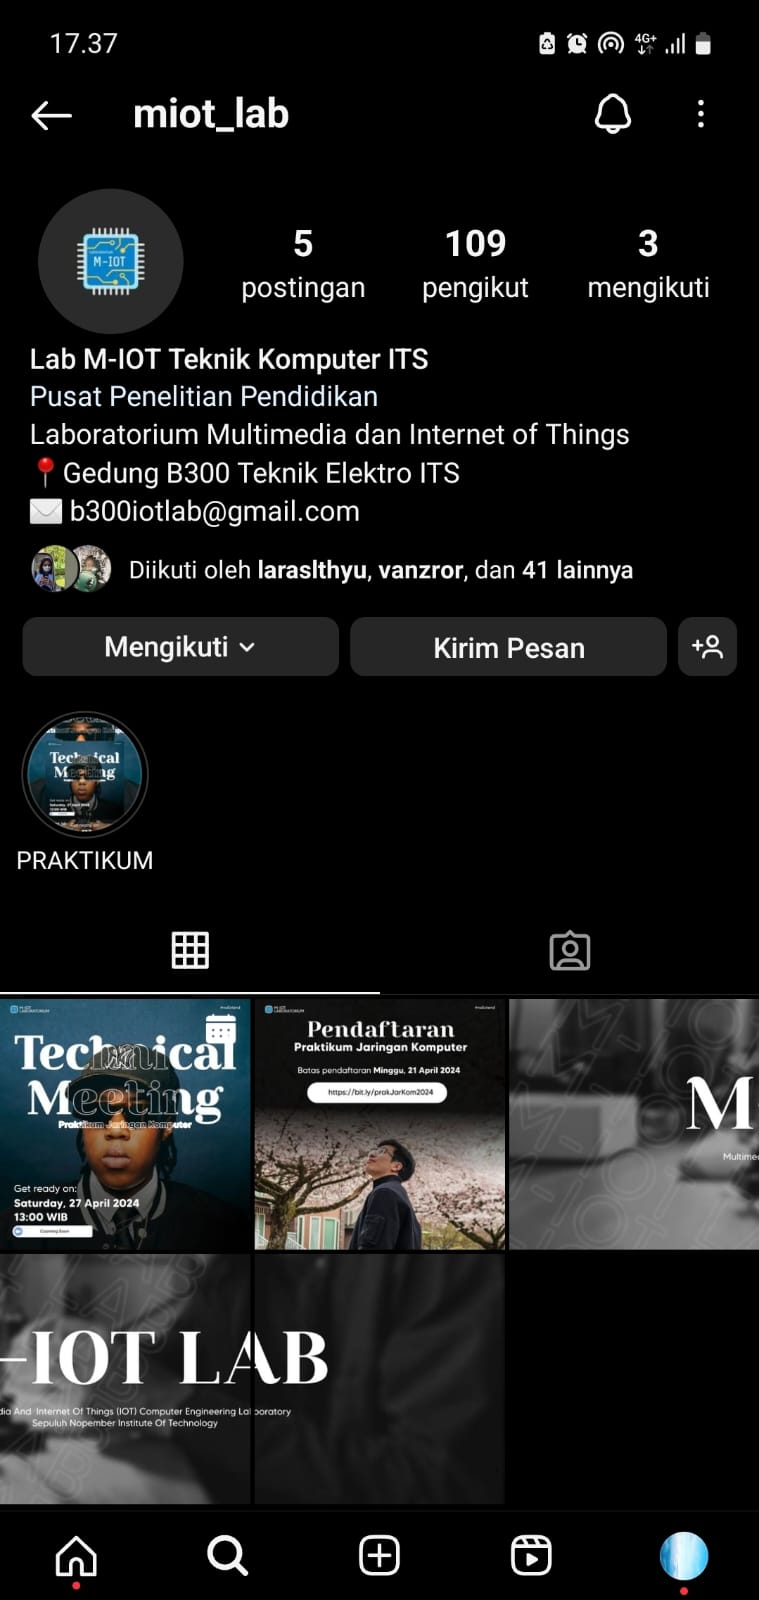
\includegraphics[width=\linewidth]{P1/img/zafafollow.jpg}
			\caption{Bukti Azaria follow}
			\label{fig:gambar36}
		\end{subfigure}
		\begin{subfigure}{0.8\linewidth}
			\centering
			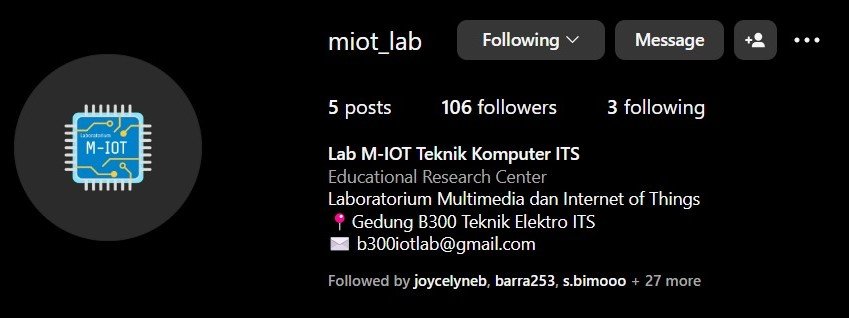
\includegraphics[width=\linewidth]{P1/img/larasfollow.jpg}
			\caption{Bukti Laras follow}
			\label{fig:gambar37}
		\end{subfigure}
		\caption{Bukti follow IG Lab MIOT}
		\label{fig:dua_gambar}
	\end{figure}
	
\end{enumerate}
\subsection{Dokumentasi saat Praktikum}

\end{document}